\documentclass[a4paper,12pt]{article}
\usepackage[english]{babel}
\usepackage[utf8]{inputenc}
\usepackage[T1]{fontenc} 

\usepackage{amsmath}
\usepackage{float}
\usepackage{geometry}
\usepackage{hyperref}
\usepackage{graphicx}
\usepackage{varwidth}
\usepackage{tikz}
\usetikzlibrary{backgrounds,arrows,calc,positioning,shapes, decorations.markings}
\usepackage{bigfoot}
\usepackage{enumitem}

\newcommand{\filterDescription}[3]{\textbf{#1}\\\emph{#2}
  \\\vspace{-0.3cm}\\
  \begin{varwidth}{50mm}#3\end{varwidth}}


\geometry{margin=2cm}
\begin{document}

\section{Introduction}

\paragraph{}
This manual aims to explain both the algorithms used in the vision and the code using it.
It is incomplete and does not pretend to document the whole code. However, it is
supposed to guide a new user of the system.

\section{Pipeline Architecture}
\paragraph{}
Image analysis is considered as a directed acyclic graph denoted as
\emph{Pipeline}, nodes are called \emph{filters} and arcs contain images.
The cut of a \emph{Pipeline} is also called \emph{Pipeline}. Even if the names
are the same, it is not possible to design various \emph{Pipeline} separately
and merging them at the end. However, we consider the whole vision loop as a set
of \emph{Pipelines} in~\ref{sec:UsedPipelines}, because it gives a better
understanding of the process.
 
\subsection{Filters}
\paragraph{}
A \emph{filter} performs a process on the given input, given some parameters.
The result of the process is usually an image. Each filter has a name which is
supposed to be unique.

\paragraph{Input}
The input of the filter is defined as a set of filters, named
\emph{dependencies}. It is possible to create a filter with multiple
\emph{dependencies} (e.g. The \verb!Diff! filter which uses two images and
produces the difference between the two). It should be possible to use
output parameters from a dependency, however it is not implemented yet in
any of the filters used.

\paragraph{Output}
As mentioned previously, the output of a filter is usually an image.
However, some filters produce information which is not directly an image.
For instance, filters which detect lines produce lines, in this case, the
output of the filter is saved inside a named parameter which is accessible
publicly.

\paragraph{Parameters}
Each filter possess a container of parameters~\footnote{See
  \verb!Parameters/ParamsContainer.hpp!}, this container can receive
parameters from various types~\footnote{See \verb!Pipeline/Filter.hpp!}.
Although there is only one parameter container, we can distinguish three
semantical types of parameters:
\begin{description}
\item[Dynamical parameter] Those parameters are generally set by
  experimentation. They are (or should be) available through sliders.
  Colors thresholds typically belong to this category.
\item[Input parameter] Those parameters are used during execution to provide
  external information. The current angle of the camera typically belong
  to this category.
\item[Output parameter] Those parameters are only read by external entities,
  they must be set during the filter process. The position of a ball candidate
  and its radius typically belongs to this category.
\end{description}

\subsection{Pipeline}
\paragraph{}
A \emph{pipeline} is a directed acyclic graph. Filters are loaded into it,
then the order of execution of the filters is automatically resolved and
stored. Each time the \emph{Pipeline} is processed, every \emph{filter}
will be processed only once, ensuring its dependencies have been
processed before.

\subsection{Serialization}
\paragraph{}
In order to avoid compiling after every modification, \emph{pipelines} and
\emph{filters} can be imported/exported from/to xml. Therefore, the whole
vision loop might be modified without recompiling any binary. It is also
possible to use two different xml files, one for orange ball and one for white
ball.
\paragraph{}
The drawbacks of this method is that errors tend to happen during execution of
the program and not at compilation time. Therefore, a particular attention has
been put on producing explicit exceptions. However, some errors might still
happen with weird messages.

\subsection{Adding a new filter}
\paragraph{}
In order to be able to instantiate Filters from xml, it was necessary to use
a factory pattern. Therefore, adding a new filter requires to register it in
a common file~\footnote{See \verb!Filter/FilterFactory.cpp!}. A default
constructor needs to be provided by every filter, specific attention must
be given to the initialization of members when using optional parameters in xml
description.


\section{\label{sec:UsedPipelines}Used Pipelines}
\paragraph{}
The whole vision system can be divided into subtasks, each of them having its
own goal.

\paragraph{}
First of all, the clipping is a task whose goal is to determine the field area.
It is used in order to avoid all the \emph{noise} which can be found outside of
the field area. Currently, there is also a ball detection using colors and
shape and a goal detection based on the vertical posts and their color.

\subsection{Clipping}
\paragraph{}
In order to avoid detecting objects outside of the game arena (e.g. a member
of the public wearing a t-shirt with a white ball). The first step toward a
robust detection is to detect the arena in order to avoid considering the
part of the world where anything might happen.
\paragraph{}
The pipeline used for clipping is described at Fig.~\ref{fig:clipping}. The
analysis is performed on a downscaled image in order to reduce computational
time. First, pixels which do not match the color of the playing field are
removed. Then, noise is filtered by opening and neighbors areas are
merged by closure. Finally the borders of the arena are detected by using
a RHT (Randomized Hough Transform) on the edges of the detected areas.
%TODO describe randomized hough transform, maybe in appendix
\paragraph{}
Some other ideas have already been explored such has:
\begin{itemize}
\item using a dynamical range for the field color, computing it from an
  histogram (based on the fact that the field color represent a major
  part of the field).
\item looking for homogeneous region by using a difference between the original
  image and blurred image (based on the fact that the content outside of the
  field is less homogeneous).
\end{itemize}
\paragraph{}
While these ideas led to satisfying results, it does not seems to be necessary.
Therefore those treatments have been removed. If using a static range for colors
is not sufficient, those methods might be used to increase the accuracy of
clipping.


\begin{figure}
  \centering
  \caption{\label{fig:clipping}Computing the clipping}
  \makeatletter
\def\getnodedistance{\tikz@node@distance}
\makeatother

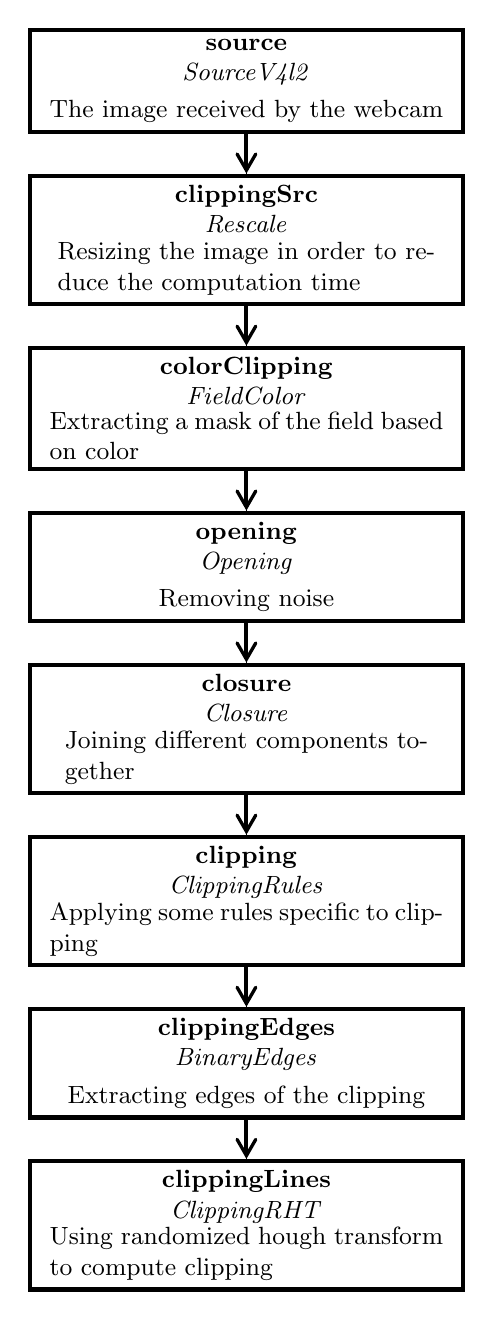
\begin{tikzpicture}[scale=0.5,node distance=5mm, >=latex',
  block/.style = {draw, rectangle, minimum height=10mm, minimum width=55mm,
    align=center, ultra thick},
  vecArrow/.style={
    decoration={markings,mark=at position
      1 with {\arrow[scale=1.5,thick]{angle 60}}},
    preaction = {decorate},
    postaction = {draw,line width=1.5pt, shorten >= 1.5pt}
  },
  font=\small]
% Source
\node[block] (source) {\filterDescription{source}{SourceV4l2}
  {The image received by the webcam}};
% ClippingSrc
\node[block] (clippingSrc) [below=of source]
     {\filterDescription{clippingSrc}{Rescale}
       {Resizing the image in order to reduce the computation time}};
\draw[vecArrow] (source) -- (clippingSrc);
% FieldColor
\node[block] (colorClipping) [below=of clippingSrc]
     {\filterDescription{colorClipping}{FieldColor}
       {Extracting a mask of the field based on color}};
\draw[vecArrow] (clippingSrc) -- (colorClipping);
% opening (to rename)
\node[block] (opening) [below=of colorClipping]
     {\filterDescription{opening}{Opening}
       {Removing noise}};
\draw[vecArrow] (colorClipping) -- (opening);
% closure (to rename)
\node[block] (closure) [below=of opening]
     {\filterDescription{closure}{Closure}
       {Joining different components together}};
\draw[vecArrow] (opening) -- (closure);
% clipping
\node[block] (clipping) [below=of closure]
     {\filterDescription{clipping}{ClippingRules}
       {Applying some rules specific to clipping}};
\draw[vecArrow] (closure) -- (clipping);
% clippingEdges
\node[block] (clippingEdges) [below=of clipping]
     {\filterDescription{clippingEdges}{BinaryEdges}
       {Extracting edges of the clipping}};
\draw[vecArrow] (clipping) -- (clippingEdges);
% clipping
\node[block] (clippingLines) [below=of clippingEdges]
     {\filterDescription{clippingLines}{ClippingRHT}
       {Using randomized hough transform to compute clipping}};
\draw[vecArrow] (clippingEdges) -- (clippingLines);
\end{tikzpicture}

\end{figure}

\subsection{Ball Detection}
\paragraph{}
A diagram describing the ball detection process is presented at
Fig.~\ref{fig:ballDetection}. The first part of the treatment identifies
regions of interest on a downscaled image. Those regions of interest are used
in the second part, where candidates for the ball are identified using a circle
detection based on the randomized hough transform.
\paragraph{}
Since the ball will be white (as lines and goals), identifying regions of
interest might be more problematic. Starting with an opening should help to
reduce the risks of identifying lines as regions of interest, because ball is
thicker than the lines, however it will make detecting the ball from far less
realistic.
\paragraph{}
Before applying an expensive treatment, 4 different filters are used to reject 
ROI which are not susceptible of containing the ball.
\begin{enumerate}
\item ROI must have a similar width and height, because the bounding box of a
  circle is a square. This condition rejects most of the lines because their
  bounding box is very different from a square.
\item The size of the bounding box must be coherent with the tilt of its center.
  It is ridiculous to use a large ROI at the horizon or in the opposite case, a
  tiny ROI when the robot is looking at his feet.
\item There must be at least some pixels with a very high brightness because the
  ball is almost spheric and therefore, it always reflects light.
\item There must be at least some pixels with a very low brightness because the
  ball will project shadow on the ground.
\end{enumerate}


\begin{figure}
  \centering
  \caption{\label{fig:ballDetection}Computing the ballDetection}
  \makeatletter
\def\getnodedistance{\tikz@node@distance}
\makeatother

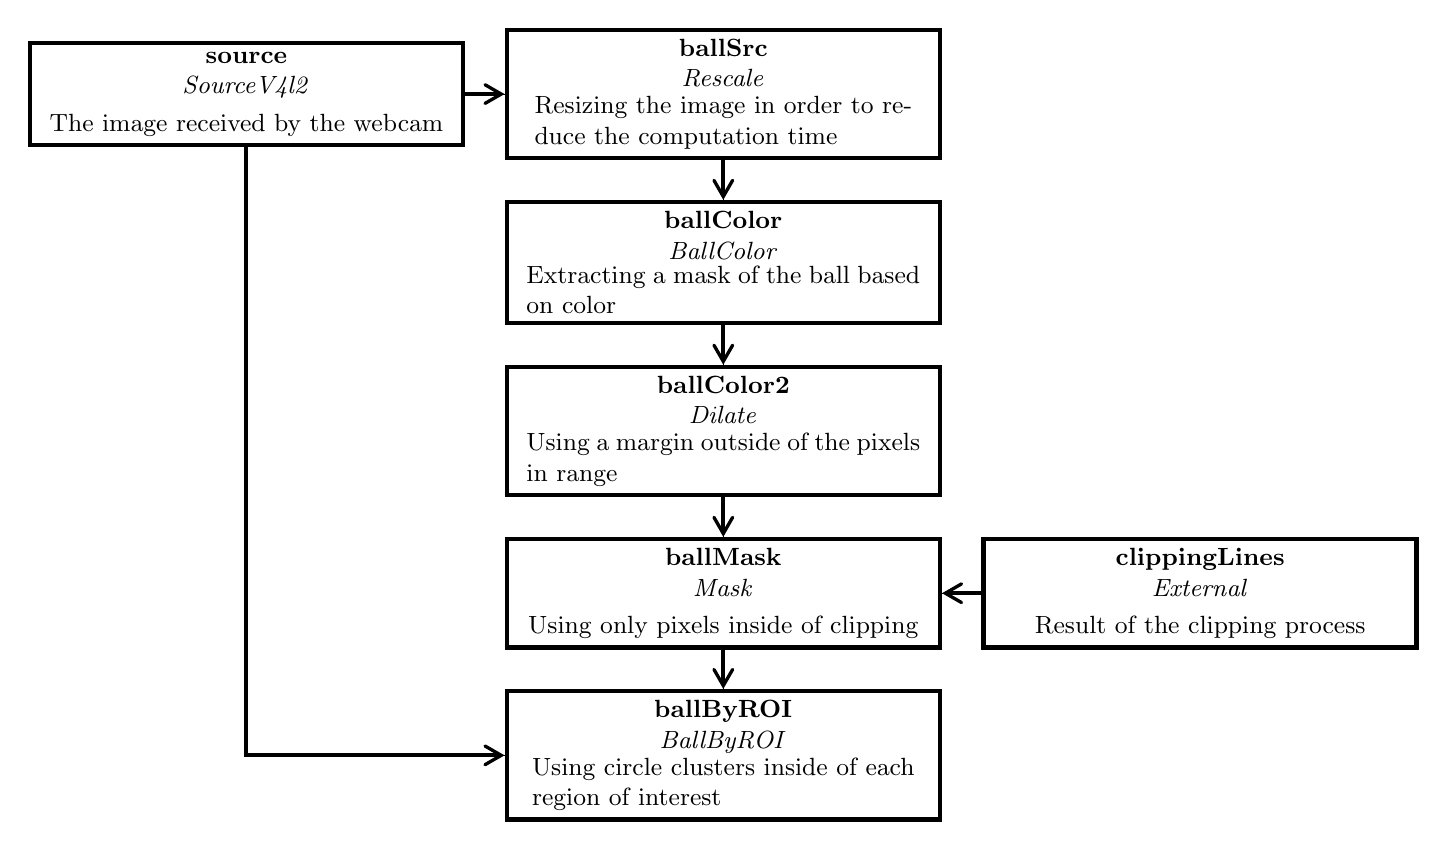
\begin{tikzpicture}[scale=0.5,node distance=5mm, >=latex',
  block/.style = {draw, rectangle, minimum height=10mm, minimum width=55mm,
    align=center, ultra thick},
  vecArrow/.style={
    decoration={markings,mark=at position
      1 with {\arrow[scale=1.5,thick]{angle 60}}},
    preaction = {decorate},
    postaction = {draw,line width=1.5pt, shorten >= 1.5pt}
  },
  font=\small]
% Source
\node[block] (source) {\filterDescription{source}{SourceV4l2}
  {The image received by the webcam}};
% ClippingSrc
\node[block] (ballSrc) [right=of source]
     {\filterDescription{ballSrc}{Rescale}
       {Resizing the image in order to reduce the computation time}};
\draw[vecArrow] (source) -- (ballSrc);
% BallColor
\node[block] (ballColor) [below=of ballSrc]
     {\filterDescription{ballColor}{BallColor}
       {Extracting a mask of the ball based on color}};
\draw[vecArrow] (ballSrc) -- (ballColor);
% BallColor2
\node[block] (ballColor2) [below=of ballColor]
     {\filterDescription{ballColor2}{Dilate}
       {Using a margin outside of the pixels in range}};
\draw[vecArrow] (ballColor) -- (ballColor2);
% BallMask
\node[block] (ballMask) [below=of ballColor2]
     {\filterDescription{ballMask}{Mask}
       {Using only pixels inside of clipping}};
\draw[vecArrow] (ballColor2) -- (ballMask);
\node[block] (clippingLines) [right=of ballMask]
     {\filterDescription{clippingLines}{External}
       {Result of the clipping process}};
\draw[vecArrow] (clippingLines) -- (ballMask);
% BallByROI
\node[block] (ballByROI) [below=of ballMask]
     {\filterDescription{ballByROI}{BallByROI}
       {Using circle clusters inside of each region of interest}};
\draw[vecArrow] (ballMask) -- (ballByROI);
\draw[vecArrow] (source) |- (ballByROI);
\end{tikzpicture}

\end{figure}

\subsection{Goal Detection}
TODO describe

\begin{figure}
  \centering
  \caption{\label{fig:goalDetection}Computing the goalDetection}
  \makeatletter
\def\getnodedistance{\tikz@node@distance}
\makeatother

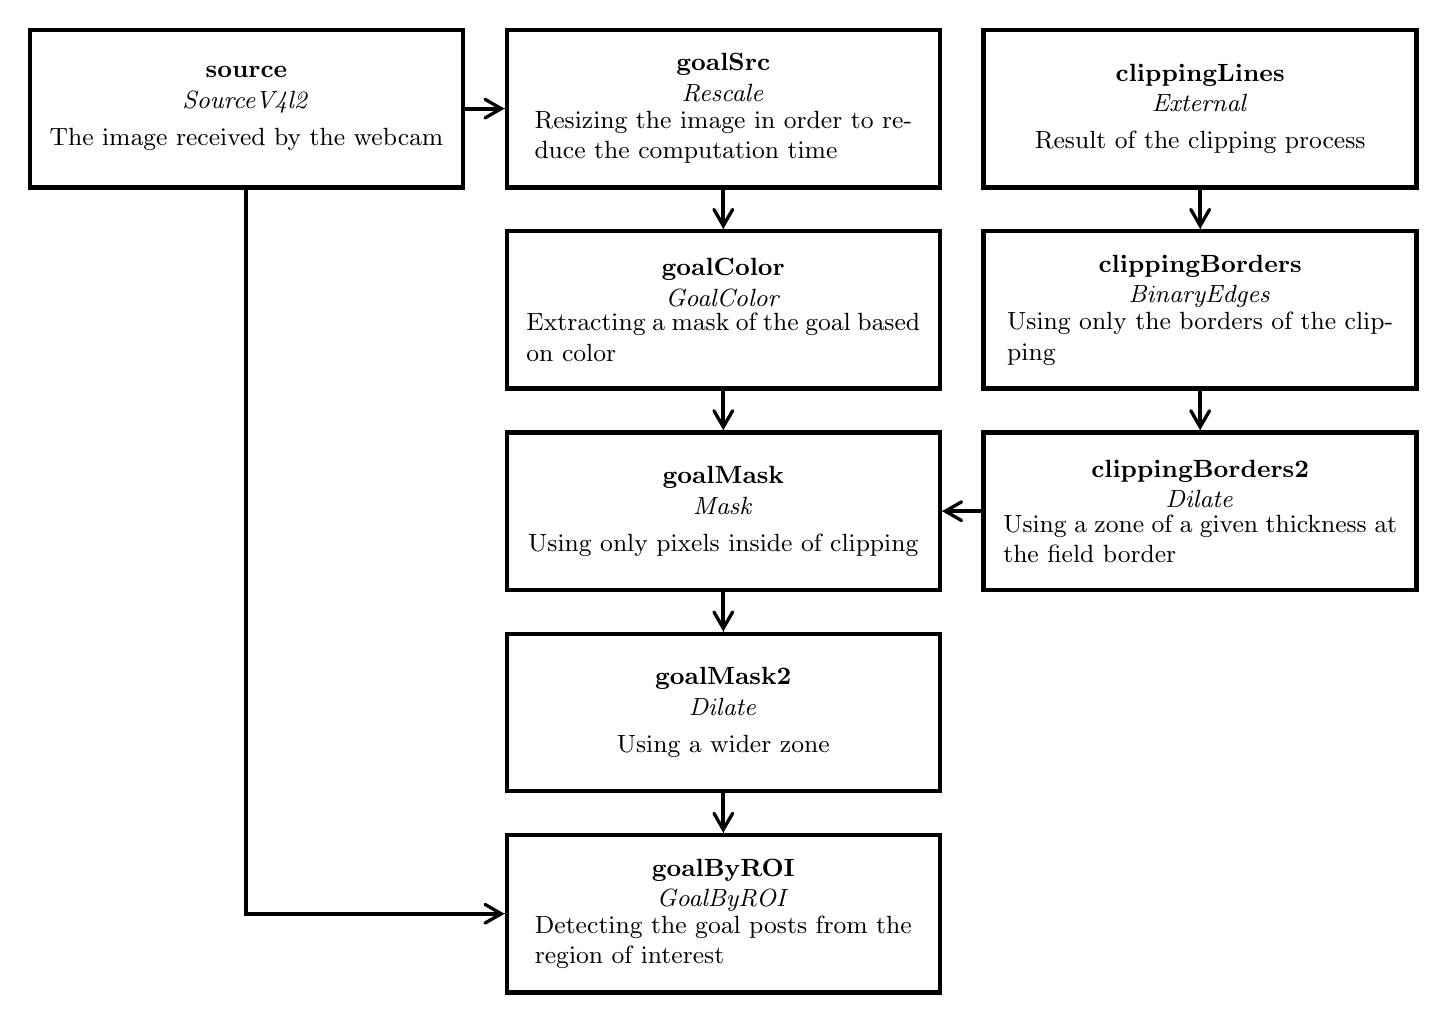
\begin{tikzpicture}[scale=0.5,node distance=5mm, >=latex',
  block/.style = {draw, rectangle, minimum height=20mm, minimum width=55mm,
    align=center, ultra thick},
  vecArrow/.style={
    decoration={markings,mark=at position
      1 with {\arrow[scale=1.5,thick]{angle 60}}},
    preaction = {decorate},
    postaction = {draw,line width=1.5pt, shorten >= 1.5pt}
  },
  font=\small]
% Source
\node[block] (source) {\filterDescription{source}{SourceV4l2}
  {The image received by the webcam}};
% goalSrc
\node[block] (goalSrc) [right=of source]
     {\filterDescription{goalSrc}{Rescale}
       {Resizing the image in order to reduce the computation time}};
\draw[vecArrow] (source) -- (goalSrc);
% GoalColor
\node[block] (goalColor) [below=of goalSrc]
     {\filterDescription{goalColor}{GoalColor}
       {Extracting a mask of the goal based on color}};
\draw[vecArrow] (goalSrc) -- (goalColor);
% GoalMask
\node[block] (goalMask) [below=of goalColor]
     {\filterDescription{goalMask}{Mask}
       {Using only pixels inside of clipping}};
\draw[vecArrow] (goalColor) -- (goalMask);
% Clipping part
\node[block] (clippingLines) [right=of goalSrc]
     {\filterDescription{clippingLines}{External}
       {Result of the clipping process}};
\node[block] (clippingBorders) [below=of clippingLines]
     {\filterDescription{clippingBorders}{BinaryEdges}
       {Using only the borders of the clipping}};
\draw[vecArrow] (clippingLines) -- (clippingBorders);
\node[block] (clippingBorders2) [below=of clippingBorders]
     {\filterDescription{clippingBorders2}{Dilate}
       {Using a zone of a given thickness at the field border}};
\draw[vecArrow] (clippingBorders) -- (clippingBorders2);
\draw[vecArrow] (clippingBorders2) -- (goalMask);
% GoalMask2
\node[block] (goalMask2) [below=of goalMask]
     {\filterDescription{goalMask2}{Dilate}
       {Using a wider zone}};
\draw[vecArrow] (goalMask) -- (goalMask2);
% GoalByROI
\node[block] (goalByROI) [below=of goalMask2]
     {\filterDescription{goalByROI}{GoalByROI}
       {Detecting the goal posts from the region of interest}};
\draw[vecArrow] (goalMask2) -- (goalByROI);
\draw[vecArrow] (source) |- (goalByROI);
\end{tikzpicture}

\end{figure}

\subsection{Adversaries Detection}
Not implemented yet.

\section{Localisation}
\paragraph{}
While the \emph{vision} module tries to extract information from an image such
as the ball position, the \emph{localisation} module tries to filter information
coming from the vision, and the lowlevel (i.e. sensors and motors). Ideally, the
information coming from the referee and from the walking loop should be taken
into account, but it is actually not implemented.
\paragraph{}
Since the information received by the \emph{localisation} module is subject to
noise as well as false positive and false negatives, we use particle filters.
The main advantage over kalman filter being that it can model a distribution
much closer to the reality than a gaussian distribution, for instance a
distribution with several candidates.

\subsection{Timing issues}
\paragraph{}
One of the main problems for producing meaningfull information is that the
localisation is based on different sources of information which have
different delays. Therefore, we use Timestamps to synchronize all the
information. Since the camera is the source of information with the highest
delay, we choosed to base the Timestamp of the localisation on the timestamp
provided by the camera. In order to get an accurate model of the robot, it is
therefore necessary to obtain the state of the robot (mainly the position and
orientation of the camera) at the moment the image was taken.
\paragraph{}
When another module requests information from the particle filter, there are
solutions which reduce the delay of the information. Currently, we
use information posterior to the last analyzed image to update the model
(e.g. if the LowLevel sent information indicating that the robot turned since
the last analyzed image, the position of the ball will be rotated of the angle
given by the Lowlevel).
\paragraph{}
After several experiments at various frequency, the delay of the camera is
approximately 30 milliseconds.

\subsection{Storing lowlevel information}
\paragraph{}
The main information needed from LowLevel are the position and the orientation
of the camera. In order to reconstruct the camera orientation at the time
when the image was taken, we request information to the lowlevel at 50 Hz and
store them in a queue containing the last $n$ information.
\paragraph{}
Since working on vision requires taking logs and working on logs, we use an
abstract class (i.e. \verb!CameraStateProvider!), this allows us to use two
different subclasses, one for embedded situations and one for playing logs. In
order to reduce the need of compilation, this choice is indicated in the xml
file.

\subsection{Ball localisation}
\paragraph{}
In this part, we explain how the mutation of the ball particles is performed,
which observations are used, why we need to use resampling and how the ball
speed is estimated.
%TODO define particles
\paragraph{}
There is two main difficulties concerning the ball localisation. The first is
to ensure that when there is no ball observation during a long time, the next
ball observation will have a real effect. Therefore, the stationary
distribution should be mostly similar to an uniform distribution on pan and tilt
angles to the ball. The second problem is to ensure that when the ball is moving
in the robot basis, particle will be moving at an approximately equivalent
speed. If the ball exploration depends strictly on pan and tilt, the ball
exploration in the cartesian space will be almost null. We can see that it is
necessary to find an equilibrium between these two problems.

\paragraph{Mutation}
The ball is always located in the robot basis, and coordinates of the ball are
defined by the pan and tilt angle since it is the space of observation. The
exploration is composed of a gaussian noise added to the pan and the tilt of the
particles, and a gaussian noise added to the cartesian position of the
particles. The controlled part of the mutation is based on two different input.
The first is the difference of orientation given by the compass or the
integration of the gyroscope. The second is the estimated speed of the ball
which is obtained by a process explained in~\ref{sec:SpeedEstimator}.

\paragraph{Observations used}
There is three types of observation used in the particle filter. The first is a
static observation used to destroy particles which are located at a distance
higher than 16 meters from the robot. The second observation is the position of
the ball which affect the score using a sigmoid function of the error and
considering a false positive rate. The third observation type is more
complicated, it consists of using the fact that the ball was not seen inside the
image while it should have been seen according to the particle. While this helps
to increase the particle density in areas which have not been checked recently,
it brings a major problem: when the ball is hidden behind a robot, the
particle's scores are reduced. Using this observation results with a loss of
memory because the particles placing the ball outside of the robots field of
view have a higher score than the other

\paragraph{Resampling}
Using a low exploration allows to increase the stability of the filter even when
he does not receive more information. However, if the ball has moved while the
robot was looking somewhere else, the particles will take a long time to
converge to the new position of the ball. Resampling partially solves this
problem by taking a few particles at each step and randomizing their position
with an uniform distribution among the state space.

\paragraph{\label{sec:SpeedEstimator}Speed estimator}
Adding the ball speed as dimensions of the particles would require to increase
the number of particles needed. In order to estimate the speed of the ball, we
use the last estimations of the ball position and their quality (i.e. a score
in $[0,1]$ based on the dispersion of the particles). In order to reduce the
delay induced by filtering, more recent values have a higher weight than old
values on the final estimation. A score is also given to the final estimation
of the speed, using dispersion of speeds.

\paragraph{External events}
When the robot is lifted or falls, the filter should be initialized again,
resampled or the exploration rate should be highly increased. The most
adaptative way to do it is to offer a service, allowing other modules to
act on the ballState.

\subsection{Robot localisation}
\paragraph{}
In this part, we present various parts of the robot localisation such as the
rules for particle mutations and the observations used.
\paragraph{}
The particles used for robot localisation are composed of three parameters:
\begin{itemize}
\item the x coordinate on the field,
\item the y coordinate on the field,
\item the orientation of the robot body.
\end{itemize}

\paragraph{Mutation}
The mutation of the robot is currently composed of:
\begin{itemize}
  \item Gaussian noise on the position $\{x,y\}$ and on the robot orientation.
  \item A controlled mutation based on the integration of the gyroscope.
\end{itemize}
We also could add a basic version of odometry, based on information provided
by the walk module.

\paragraph{Observations}
There are actually 4 types of observations used for the robot localisation.
\begin{description}[labelindent=1cm, leftmargin=4.5cm, style=sameline]
\item[Field:] This observation immediately reject any particle outside of the
  playing field. While it does not fit the reality (robot might be temporarily
  outside of the playing field). It removes the risk of converging to a solution
  which is entirely outside of the field.
\item[Compass:] After the RoHOW event, it has been clear that the lack of
  accuracy from the compass could be really high. However, it is still the
  only available solution to determine which goal the robot is facing.
  Therefore, the information provided by the compass decreases the score of
  particles only when the difference between the particle and the observation
  value is very high. Therefore it can almost be considered as a binary
  information.
\item[Goal:] The vision loop produces observations corresponding to the base of
  goal posts. In order to calculate the score of a particle, we calculate the
  difference between the position in the image and the expectation according to
  the particle. This process is repeated for each post, in order to
  consider only the best option for the particle. The current algorithm considers
  all the goal observations are independant. Thus, if two posts are seen in a
  single image, they can be considered twice as the same object. While this
  seems to be a problem, it reduces the impact of false positive from goal
  detection and keeps the code simple.
\item[ArenaCorners:] When the clipping detects more than one line, intersections
  of the detected lines represent points which are the corner of the playing
  arena (i.e. the area covered with grass). The score of those observations is
  currently computed in a similar fashion as those of the goal.
\end{description}



\section{Monitoring}
\paragraph{}
In order to develop properly the vision module and to understand the problems
when the vision loop runs on the robot, it is crucial to display information
properly. Therefore, efforts have been made to provide an interface allowing to
find the source of the problem quickly.

\subsection{Execution time}
\paragraph{}
The time required for a step of the vision loop should remain reasonable. Since
we use a pipeline architecture, it is particularly important to know which steps
are consuming most of the time. With the design we use, it is easy to monitor
the time consumption along with the source of time consumption wihout needing
to compile again the binary. The only modification required is to turn the
\verb!benchmark! flag to \verb!true! in the xml file. The level of detail is
specified by the flag \verb!benchmarkDetail!, the value used defines the depth
of the benchmark tree to be displayed.

\subsection{Filter results}
\paragraph{}
When developping or tunning a pipeline, we often need to display the result of a
given filter

\subsection{Robot view}
\subsection{Field view}
\subsection{Tagged image}


\section{Checklist}

\paragraph{}
When encountering a new environment, several things must be checked/tuned. Here,
we present an ordered list of the thing to do.

\begin{enumerate}
\item Tuning the parameters of the camera
\item Ensuring that the clipping is properly detected
\item Checking the ball detection
\item Checking the ball tracking
\item Checking the goal detection
\item Checking field localisation
\end{enumerate}

\subsection{Tuning cameras parameters}
TODO describe procedure
\subsection{Checking clipping}
TODO describe test and expected results
\subsection{Checking ball detection}
TODO describe test and expected results
\subsection{Checking ball tracking}
TODO describe test and expected results
\subsection{Checking goal detection}
TODO describe test and expected results
\subsection{Checking field localisation}
TODO describe test and expected results

\end{document}
